\documentclass{beamer}

\usefonttheme{professionalfonts} % using non standard fonts for beamer
\usefonttheme{serif} % default family is serif

\usepackage{hyperref}

%\usepackage{minted}

\usepackage{animate}

\usepackage{graphicx}

\def\Put(#1,#2)#3{\leavevmode\makebox(0,0){\put(#1,#2){#3}}}

\usepackage{color}

\usepackage{tikz}

\usepackage{amssymb}

\usepackage{enumerate}


\newcommand\blfootnote[1]{%

  \begingroup

  \renewcommand\thefootnote{}\footnote{#1}%

  \addtocounter{footnote}{-1}%

  \endgroup

}

\makeatletter

%%%%%%%%%%%%%%%%%%%%%%%%%%%%%% Textclass specific LaTeX commands.

 % this default might be overridden by plain title style

 \newcommand\makebeamertitle{\frame{\maketitle}}%

 % (ERT) argument for the TOC

 \AtBeginDocument{%

   \let\origtableofcontents=\tableofcontents

   \def\tableofcontents{\@ifnextchar[{\origtableofcontents}{\gobbletableofcontents}}

   \def\gobbletableofcontents#1{\origtableofcontents}

 }

%%%%%%%%%%%%%%%%%%%%%%%%%%%%%% User specified LaTeX commands.

\usetheme{Malmoe}

% or ...

\useoutertheme{infolines}

\addtobeamertemplate{headline}{}{\vskip2pt}



\setbeamercovered{transparent}

% or whatever (possibly just delete it)

\makeatother

\begin{document}
\title[Discussion 10 - Review]{CS/MATH 111, Discrete Structures - Fall 2018. \\ Discussion 10 - Review}
\author[CS111]{Andres, Sara, Elena}
\institute[Fall'18]{University of California, Riverside}
\makebeamertitle
\newif\iflattersubsect

\AtBeginSection[] {
    \begin{frame}<beamer>
    \frametitle{Outline} 
    \tableofcontents[currentsection]  
    \end{frame}
    \lattersubsectfalse
}

\AtBeginSubsection[] {
    \begin{frame}<beamer>
    \frametitle{Outline} 
    \tableofcontents[currentsubsection]  
    \end{frame}
}

\section{Problem 1}

\begin{frame}{Problem 1}
    \begin{itemize}
        \item For pseudo-code below, tell what is the number of words printed if the input is $n$. Give a recurrence and then its solution(use $\Theta$ notation). 
    \end{itemize}
    \centering 
    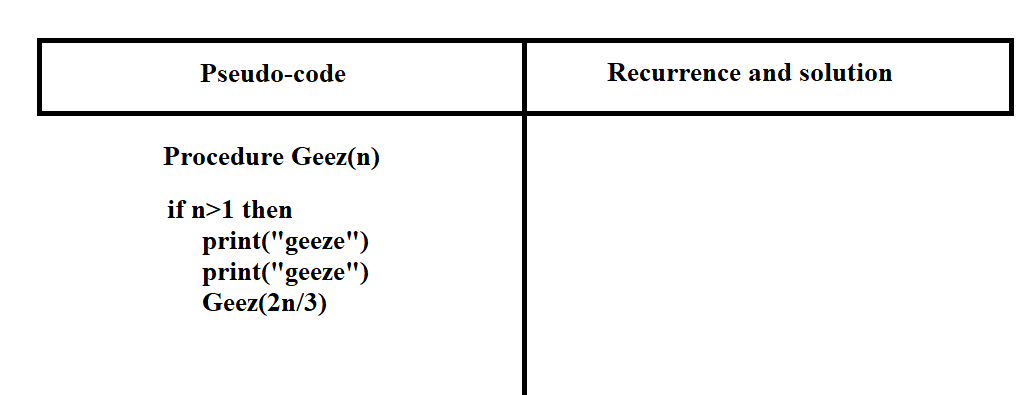
\includegraphics[width=.7\linewidth]{p1.png} 
\end{frame}

\begin{frame}{Master theorem}
    \centering
    \begin{theorem}\label{theo:master}
        Let $a \geq 0$, $b > 0$, $c > 0$ and $d \geq 0$.  If $T(n)$ satisfies the recurrence then
        $$ T(n) = a \cdot T \Big(\frac{n}{b}\Big) + c \cdot n^d $$
    \end{theorem}
    
    $T(n) =$ 
    \Bigg\{
    \begin{tabular}{l r r}
        $\Theta (n^{\log_b a})$ & \hspace{1cm} & $a > b^d$ \\
        $\Theta (n^d \log n)$   & \hspace{1cm} & $a = b^d$ \\
        $\Theta (n^d)$          & \hspace{1cm} & $a < b^d$ 
    \end{tabular}
\end{frame}

\begin{frame}{Problem 1}
   \begin{itemize}
        \item Solution:
            $T(n) = T(2n/3) + 2$
            \\ $a = 1, b = \frac{3}{2}, c = 2, d = 0$
            \\ Case 2: $n^0 \cdot log(n) = log(n)$
       \item Other examples: \url{http://people.csail.mit.edu/thies/6.046-web/master.pdf}      
    \end{itemize}
\end{frame}

\section{Problem 2}

\begin{frame}{Problem 2}
   \begin{itemize}
          \item  For any integer $x>4$, it is not possible that all three numbers $x$, $x + 2$ and $x + 4$ are prime.
      \end{itemize}
\end{frame}

\begin{frame}{Problem 2}
   \begin{itemize}
        \item  Solution:
        \begin{itemize}
            \item Since $x$ is greater than 4 it cannot be divisible by 3. So, $x$ is either in the form of $3q + 1$ or $3q + 2$ .
            \item If $x = 3q + 1$ then: $$x + 2 = 3q + 1 + 2 = 3q + 3 = 3(q + 1) = 3q^{'}$$ hence $x + 2$ is divisible by 3. Therefore, it is not a prime number.
            \item If $x = 3q + 2$ then: $$x + 4 = 3q + 2 + 4 = 3q + 6 = 3(q + 2) = 3q^{'}$$ hence $x + 4$ is divisible by 3. Therefore, it is not a prime number.
        \end{itemize}
    \end{itemize}
\end{frame}

\section{Problem 3}

\begin{frame}{Problem 3}
   \begin{itemize}
          \item Prove that $1+3+5+...+(2n-1)=n^2$ for any integer $n \geq 1$. (The expression on the left-hand-side is the sum of the first n odd natural numbers). You can use mathematical induction or any other proof method.
      \end{itemize}
\end{frame}
\begin{frame}{Problem 3}
   \begin{itemize}
        \item Solution:
        \begin{itemize}
            \item Base case: $$1 = 1^2$$
            \item Assumption: $$1 + 3 + 5 + \cdots + (2k - 1) = k^2$$
            \item Induction:    $$1 + 3 + 5 + \cdots + (2(k + 1) - 1) = (k + 1)^2$$
                                $$1 + 3 + 5 + \cdots + (2k - 1) + (2k + 1) = (k + 1)^2$$
                                $$k^2 + (2k + 1) = (k + 1)^2$$
                                $$k^2 + 2k + 1 = k^2 + 2k + 1$$
        \end{itemize}
    \end{itemize}
\end{frame}

\section{Problem 4}

\begin{frame}{Problem 4}
    \begin{itemize}
        \item Explain how the RSA cryptosystem works
    \end{itemize}
\end{frame}

\begin{frame}{Problem 4}
    \begin{itemize}
        \item Solution:
    \end{itemize}
    \centering 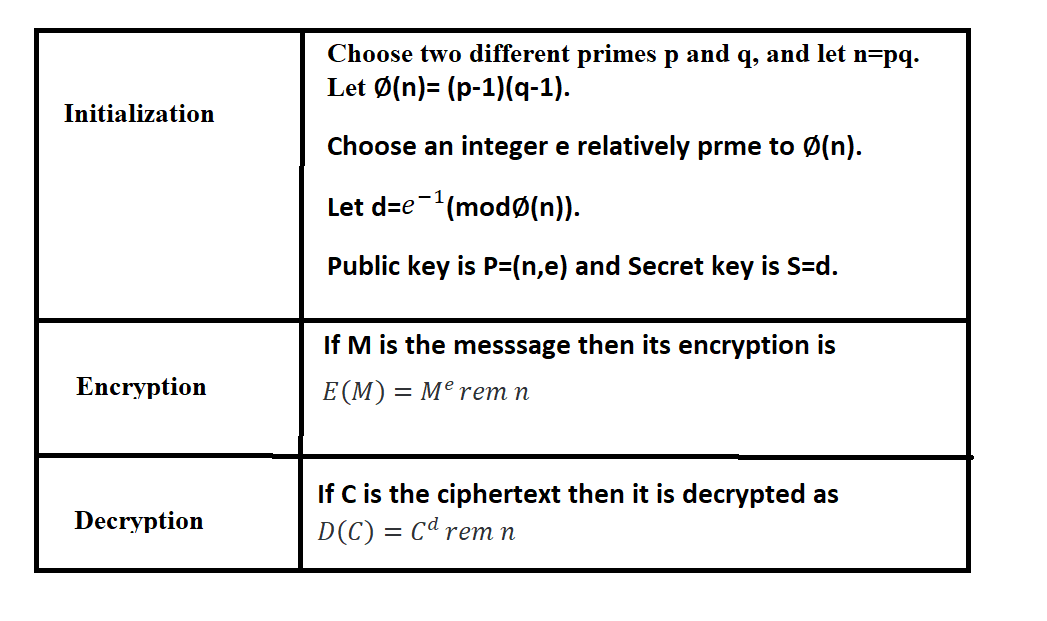
\includegraphics[width=.7\linewidth]{p2.png} 
\end{frame}

\begin{frame}{Problem 4}
    \begin{itemize}
        \item Below you are given five choices of parameters p,q,e,d of RSA. For each choice tell whether these parameters are correct. If not, give a brief justification.
    \end{itemize}
    \centering 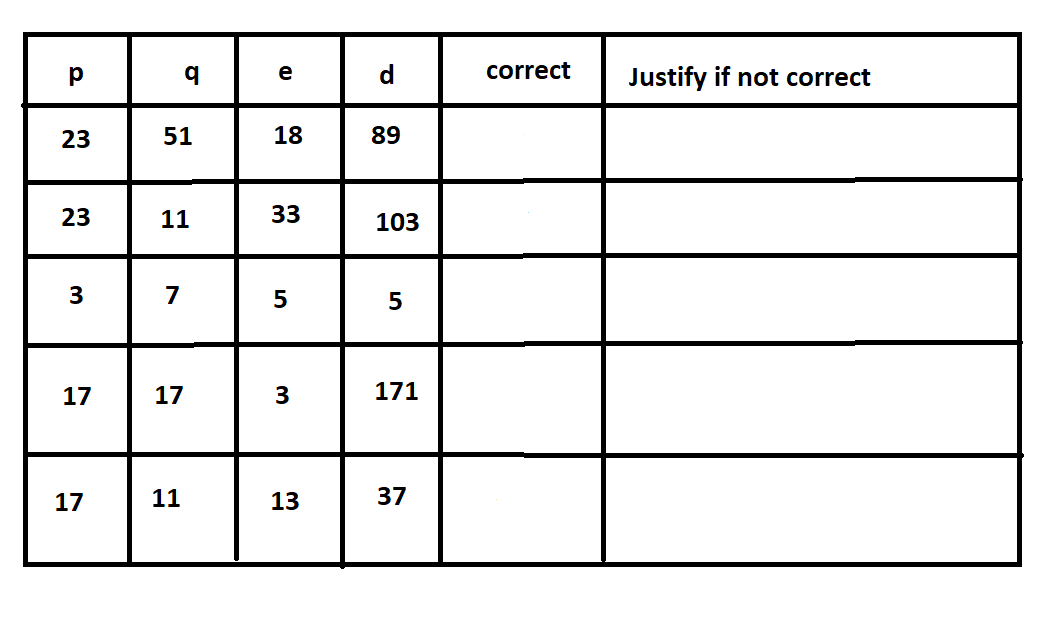
\includegraphics[width=.7\linewidth]{p4.png} 
\end{frame}

\begin{frame}{Problem 4}
    \begin{itemize}
        \item Solution:
    \end{itemize}
    \centering 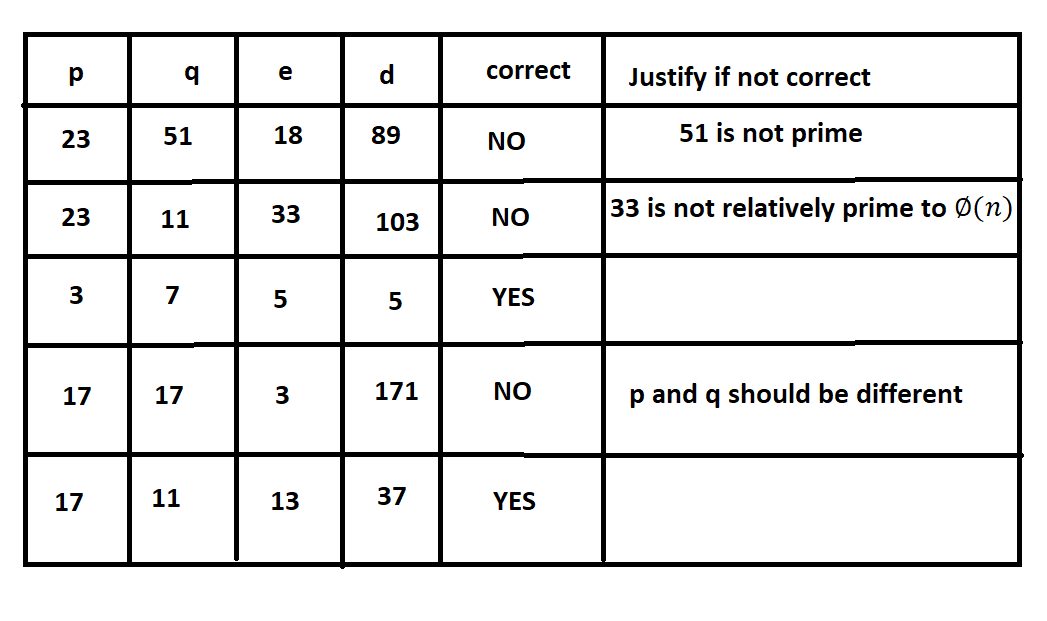
\includegraphics[width=.8\linewidth]{p3.png} 
\end{frame}

\section{Problem 5}

\begin{frame}{Problem 5}
    \begin{itemize} 
        \item Use Fermat's Little theorem to compute the following values:
        \begin{itemize}
            \item $78^{112} \pmod{113}$
            \item $3^{39635} \pmod{31}$
        \end{itemize}
    \end{itemize}
\end{frame}

\begin{frame}{Problem 5}
    \begin{itemize} 
        \item Use Fermat's Little theorem\footnote{$a^{p - 1} \equiv 1 \pmod{p}$} to compute the following values:
        \begin{itemize}
            \item $78^{112} \pmod{113} \equiv 1 \pmod{113}$
            \item $3^{39635} \pmod{31}  = 3^{30 * 1321 + 5} \pmod{31} = (3^{30})^{1321}\times3^5 \pmod{31}$ \\
                                        \hspace{2.6cm}$\equiv (1)^{1321}\times3^5 \pmod{31}$ \\
                                        \hspace{2.6cm}$\equiv 243 \pmod{31}$ \\
                                        \hspace{2.6cm}$\equiv 26 \pmod{31}$ 
        \end{itemize}
    \end{itemize}
\end{frame}

\section{Problem 6}

\begin{frame}{Problem 6}
   \begin{itemize} 
        \item Kevin is planning a 32-day trip to Scandinavia. He wants to spend at least 3 days in Finland, then between 7 and 14 days in Sweden, and later between 6 and 11 days in Norway. Compute the number of possible itineraries for his trip.
    \end{itemize}
\end{frame}

\begin{frame}{Problem 5}
    \begin{itemize} 
        \item Dealing with lower and upper bounds:
        \begin{itemize}
            \item $7\leq S \leq14$, $S^{'}=S-7$, \\ 
                    $0\leq S^{'} \leq7$
            \item $ 6\leq N \leq 11$ , $N^{'}=N-6$, \\ 
                    $0\leq N^{'} \leq5$
            \item $3\leq F \implies 3\leq F \leq 32-7-6 \implies 3\leq F \leq 19$, $F^{'} = F - 3$, \\
                    $0 \leq F^{'} \leq 16$
        \end{itemize}
        \item Stating new relations:
        \begin{itemize}
            \item $S + N + F = 32$
            \item $\implies S^{'} + 7 + N^{'} + 6 + F^{'} + 3 = 32$
            \item $\implies S^{'} + N^{'} + F^{'} = 16$
        \end{itemize}
    \end{itemize}
\end{frame}

\begin{frame}{Problem 5}
    \begin{itemize} 
        \item Applying Inclusion-Exclusion theorem:
        \begin{itemize}
            \item $S = S_{total} - S(S^{'} \geq 8 \cup N^{'} \geq 6 \cup F^{'} \geq 17)$
            \item $S = S_{total} - (S(F^{'} \geq 17) + S(S^{'} \geq 8) + S(N^{'} \geq 6) -$ \\
                    $S(F^{'} \geq 17 \cap S^{'} \geq 8) - S(F^{'} \geq 17 \cap N^{'} \geq 6) - S(N^{'} \geq 6 \cap S^{'} \geq 8) +$ \\
                    $S(F^{'} \geq 17 \cap S^{'} \geq 8 \cap N^{'} \geq 6))$
            \item $S = {16 + 3 - 1 \choose 3 - 1} - (0 - {16 - 8 - 3 - 1 \choose 3 - 1} - {16 - 6 - 3 - 1 \choose 3 - 1} + 0 + 0 + {16 - 14 + 3 - 1 \choose 3-1} -0)$
        \end{itemize}
    \end{itemize}
\end{frame}

\end{document}
